\documentclass[10pt]{article}  

%%%%%%%% PREÁMBULO %%%%%%%%%%%%
\title{Plantilla para reportes IMEC-UTB}
\usepackage[spanish]{babel} %Indica que escribiermos en español
\usepackage[utf8]{inputenc} %Indica qué codificación se está usando ISO-8859-1(latin1)  o utf8  
\usepackage{amsmath} % Comandos extras para matemáticas (cajas para ecuaciones,
% etc)
\usepackage{amssymb} % Simbolos matematicos (por lo tanto)
\usepackage{graphicx} % Incluir imágenes en LaTeX
\usepackage{color} % Para colorear texto
\usepackage{subfigure} % subfiguras
\usepackage{float} %Podemos usar el especificador [H] en las figuras para que se
% queden donde queramos
\usepackage{cancel}

\usepackage{capt-of} % Permite usar etiquetas fuera de elementos flotantes
% (etiquetas de figuras)
\usepackage{sidecap} % Para poner el texto de las imágenes al lado
	\sidecaptionvpos{figure}{c} % Para que el texto se alinie al centro vertical
\usepackage{caption} % Para poder quitar numeracion de figuras
\usepackage{commath} % funcionalidades extras para diferenciales, integrales,
% etc (\od, \dif, etc)
\usepackage{cancel} % para cancelar expresiones (\cancelto{0}{x})
 
\usepackage{anysize} 					% Para personalizar el ancho de  los márgenes
\marginsize{2cm}{2cm}{2cm}{2cm} % Izquierda, derecha, arriba, abajo

\usepackage{appendix}
\renewcommand{\appendixname}{Apéndices}
\renewcommand{\appendixtocname}{Apéndices}
\renewcommand{\appendixpagename}{Apéndices} 

% Para que las referencias sean hipervínculos a las figuras o ecuaciones y
% aparezcan en color
\usepackage[colorlinks=true,plainpages=true,citecolor=blue,linkcolor=blue]{hyperref}
%\usepackage{hyperref} 
% Para agregar encabezado y pie de página
\usepackage{fancyhdr} 
\pagestyle{fancy}
\fancyhf{}

\fancyhead[R]{\footnotesize División Ciencias e Ingenierías}   % dereecha
\fancyfoot[R]{\footnotesize Proyecto Final}  % Pie derecha
\fancyfoot[C]{\thepage}  % centro

\renewcommand{\footrulewidth}{0.4pt}


\usepackage{listings} % Para usar código fuente
\definecolor{dkgreen}{rgb}{0,0.6,0} % Definimos colores para usar en el código
\definecolor{gray}{rgb}{0.5,0.5,0.5} 
% configuración para el lenguaje que queramos utilizar
\lstset{language=Matlab,
   keywords={break,case,catch,continue,else,elseif,end,for,function,
      global,if,otherwise,persistent,return,switch,try,while},
   basicstyle=\ttfamily,
   keywordstyle=\color{blue},
   commentstyle=\color{red},
   stringstyle=\color{dkgreen},
   numbers=left,
   numberstyle=\tiny\color{gray},
   stepnumber=1,
   numbersep=10pt,
   backgroundcolor=\color{white},
   tabsize=4,
   showspaces=false,
   showstringspaces=false}

\newcommand{\sen}{\operatorname{\sen}}	% Definimos el comando \sen para el seno
%en español

\title{Plantilla para Reportes IMEC-UTB}
% Basada en la plantilla para reportes UPIITA de  Overleaf

%%%%%%%% TERMINA PREÁMBULO %%%%%%%%%%%%

\begin{document}

%%%%%%%%%%%%%%%%%%%%%%%%%%%%%%%%%% PORTADA %%%%%%%%%%%%%%%%%%%%%%%%%%%%%%%%%%%%%%%%%%%%
																					%%%
\begin{center}																		%%%
\newcommand{\HRule}{\rule{\linewidth}{0.5mm}}									%%%\left
 																					%%%

\begin{minipage}{0.48\textwidth} 
\centering

\includegraphics[scale = 0.3]{img/ug.jpg}
\end{minipage}

													 								%%%
\vspace*{1.0cm}								%%%
																					%%%	
\textsc{\huge Universidad de Guanajuato}\\[1.5cm]	

\textsc{\LARGE División de Ciencias \\ \vspace{5px} e Ingeniarías }\\[1.5cm]													%%%

\begin{minipage}{0.9\textwidth} 
\begin{center}																					%%%
\textsc{\LARGE Herramientas Informáticas y Gestión de la Información} \newline
\end{center}
\end{minipage}\\[0.5cm]
%%%
\begin{minipage}{0.9\textwidth} 
\begin{center}																					%%%
\textsc{\LARGE Proyecto Final}
\end{center}
\end{minipage}\\[0.5cm]    																				%%%
 			\vspace*{1cm}																		%%%
																					%%%
\HRule \\[0.4cm]																	%%%
{ \huge \bfseries Análisis de datos, jugadores de futbol Estados Unidos vs México}\\[0.4cm]	%%%
 																					%%%
\HRule \\[1.5cm]																	%%%
 																				%%%
																					%%%
\begin{minipage}{0.46\textwidth}													%%%
\begin{flushleft} \large															%%%

% Aqui a continuación pongan los nombres de los integrantes
\emph{Autor:}\\	
Juan Manuel Alvarez Paz\\

%%%
			%\vspace*{2cm}	
            													%%%
										 						%%%
\end{flushleft}																		%%%
\end{minipage}		
																%%%
\begin{minipage}{0.52\textwidth}		
\vspace{-0.6cm}											%%%
\begin{flushright} \large															%%%
\emph{Profesor:} \\																	%%%
	Alma\\
														%%%
\end{flushright}																	%%%
\end{minipage}	
\vspace*{1cm}
%\begin{flushleft}
 	
%\end{flushleft}
%%%
 																		%%%
\vspace{1cm} 



\vspace{2cm} 

\begin{center}	
Guanajuato, México \\
{\large \today}																	%%%
 			\end{center}												  						
\end{center}							 							
\newpage
Para realizar este análisis se tomó una base de datos de la plataforma \textbf{kaggle}, en dicha plataforma se encuentran los datos de mas de 18 mil jugadores y mas de 100 características de cada uno de ellos. \newline
Tras un primer filtrado encontramos que hay 340 jugadores mexicanos registrados en fifa, mientras que hay 347 jugadores estadounidenses.\cite{1}

\begin{center}
    \section*{\textbf{¿Qué país tiene los mejores jugadores?}}
\end{center}
De dicha base de datos tenemos características como nombre, edad, peso, altura, valor del jugador en euros, sueldo, puntuación general, etc. Al comparar la puntuación general vemos que en general ambos tienen jugadores de similares características, pero un cuya gráfica se observa que México tiene algunos jugadores que tienen una puntuación general mayor. 
\begin{figure}[H]
    \centering
    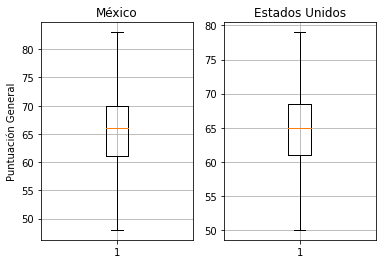
\includegraphics[scale=0.7]{latex/img/output_17_0.png}
    \caption{Distribución media de la puntuación general para México y EUA.}
    \label{fig:my_label}
\end{figure}

\begin{center}
    \section*{\textbf{¿Qué país tiene los jugadores mejor valorados?}}
\end{center}
Considerando que país tiene jugadores que valen mas de 15 millones de euros vemos que México cuenta con 5 elementos que superan por mucho dicho valor, mientras que EUA solo cuenta con un jugador que supera dicho valor.
\begin{figure}[H]
    \centering
    \subfigure[México]{   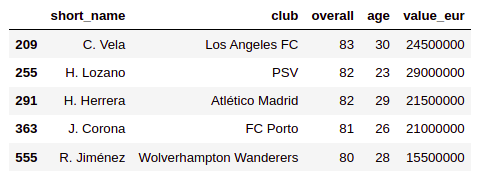
\includegraphics[scale=0.5]{latex/img/mv mex.png}}
    \subfigure[Estados Unidos]{   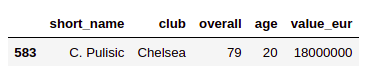
\includegraphics[scale=0.5]{latex/img/mv eua.png}}
    \label{fig:my_label}
    \caption{Jugaodres mas valuados de México y EUA.}
\end{figure}
\newpage
\begin{center}
    \section*{\textbf{Relación frecuencia y valor del jugador}}
\end{center}
Aquí podemos ver como se encuentra distribuido el valor de cada jugador, de tal manera que encontramos una frecuencia en dicho valor, de tal manera que obtenemos la siguiente distribución.
\begin{figure}[H]
    \centering
    \subfigure[México]{   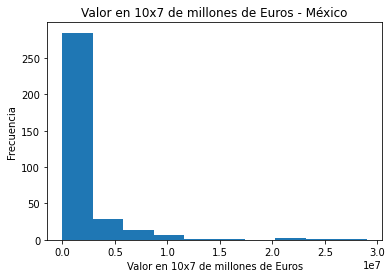
\includegraphics[scale=0.55]{latex/img/output_24_1.png}}
    \subfigure[Estados Unidos]{   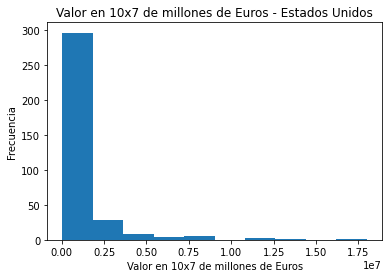
\includegraphics[scale=0.55]{latex/img/output_29_1.png}}
    \label{fig:my_label}
    \caption{Frecuencia en el valore de los  jugadores.}
\end{figure}
Como se pudo observar en la figura anterior, para ambos países la mayoría de sus jugadores se encuentran en un valor menor a los 5 millones de euros, y solo unos cuantos superan dicha cifra. \newline
\begin{center}
    \section*{\textbf{Relación entre edad y valoración}}
\end{center}
Existe una idea de que entre más grande sea un jugador se rendimiento será menor, lo que se pretende observar aquí es cómo es que el rendimiento de los jugadores cambia con respecto a su edad.
\begin{figure}[H]
    \centering
    \subfigure[México]{   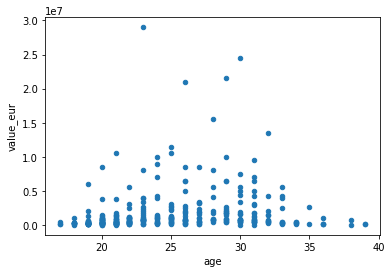
\includegraphics[scale=0.55]{latex/img/output_34_1.png}}
    \subfigure[Estados Unidos]{   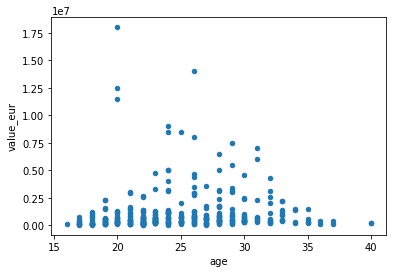
\includegraphics[scale=0.55]{latex/img/output_36_1.png}}
    \label{fig:my_label}
    \caption{Relación valor jugador y edad.}
\end{figure}
Podemos observar que el rango de edad óptimo lo encontramos entre los 20 y 33 años de edad. \newpage

\begin{center}
    \section*{\textbf{Cómo han evolucionado los mejores jugadores de México?}}
\end{center}
Veamos cómo ha cambiado la valoración de los mejores jugadores a lo largo de los últimos 6 años.

\begin{figure}[H]
    \centering
    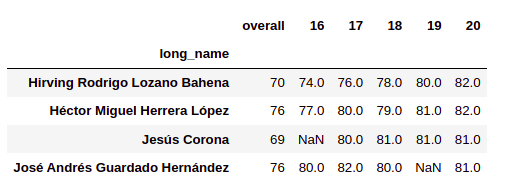
\includegraphics[scale=0.7]{latex/img/mejores mx.png}
    \caption{Los mejores jugadores de México del 2020.}
    \label{fig:my_label}
\end{figure}

Hemos visto que  todos los  jugadores mejoraron, desde un promedio de los 69-76 en 2015, hasta un valor de entre 80 y 81, los  que quiere decir que desde el 2015 todos ellos han mejorado profesionalmente.  
 \begin{center}
    \section*{\textbf{Conclusión}}  
 \end{center}
 

Hemos visto que México tiene una gran cantidad de jugadores, y ellos se encuentran en un gran nivel, además de la evidente mejora de los jugadores mexicanos a lo largo de los últimos 6 años.
\subsection*{Conclusión general}

El  análisis de datos se puede aplicar a una gran cantidad de áreas, desde la educación, ciencia, salid, deportes, etc. Con esta gran herramienta se pueden lograr cosas increíbles, además de agilizar una gran cantidad de procesos y por supuesto el ahorro de tiempo.

\begin{thebibliography}{}
\bibitem{1}"FIFA 20 complete player dataset", Kaggle.com, 2021. [Online]. Available: https://www.kaggle.com/stefanoleone992/fifa-20-complete-player-dataset?select=players_19.csv. [Accessed: 17- Jun- 2021].

\end{thebibliography}
\end{document}
